\chapter{Problematyka strumieniowania danych}
\label{cha:rozdzial2}

\section{Wstęp}

Poniższy rozdział skupia się na problematyce strumieniowania danych multimedialnych w sieciach komputerowych. Omawia niepożądane zjawiska występujące podczas transmisji danych oraz zmienność warunków panujących w sieciach komputerowych. Zwraca uwagę na zależność jakości i szybkości transmisji danych od konfiguracji sieci i urządzeń sieciowych oraz na zalety wykorzystania transmisji grupowych w przypadku komunikacji jeden do wielu.

\section{Zajwiska występujące podczas transmisji danych}

Aplikacje zajmujące się strumieniowaniem danych narażone są na wiele zjawisk związanych z wymianą informacji w sieciach komputerowych. Do zjawisk, które mogą spowodować największe zakłócenia podczas transmisji danych należą: opóźnienia, jitter oraz utrata danych przesyłanych przez sieć.

Opóźnienie w trakcie przesyłania danych wynika przede wszystkim z czasu transmisji danych przez media fizyczne oraz z czasu przetwarzania danych przez urządzenia sieciowe znajdujące się na trasie od nadawcy do odbiorcy. Nowoczesne urządzenia sieciowe przełączają ruch z szybkością bliską \textit{wire-speed}\footnote{Maksymalna szybkość wykorzystywanego standardu komunikacyjnego.}, wykorzystując w tym celu specjalne układy scalone \textit{ASIC}\footnote{Application Specific Integrated Circuit - układy scalone przeznaczone do wykonywania z góry ustalonego zadania.}. Kolejnym powodem występowania opóźnień jest duży ruch w sieci. Urządzenia sieciowe przetwarzające dane zwykle wykorzystują bufory znajdujące się na interfejsach w celu przechowania danych przychodzących zanim zostaną one skierowane na interfejsy wyjściowe. Jeżeli ruch przechodzący przez urządzenie jest na tyle duży, że urządzenie pracuje z maksymalną szybkością, to bufory zaczną zapełniać się danymi. Taka sytuacja prowadzi do opóźnień w transmisji - dane muszą czekać określony czas zanim zostaną przetworzone przez urządzenie. Parametr opisujący opóźnienie występujące na drodze od nadawcy do odbiorcy i z powrotem to tzw. \textit{Round Trip Time}. Do pomiaru opóźnienia może posłużyć program Ping dostępny na większości systemów operacyjnych.

\begin{figure}[h!]
	\centering
		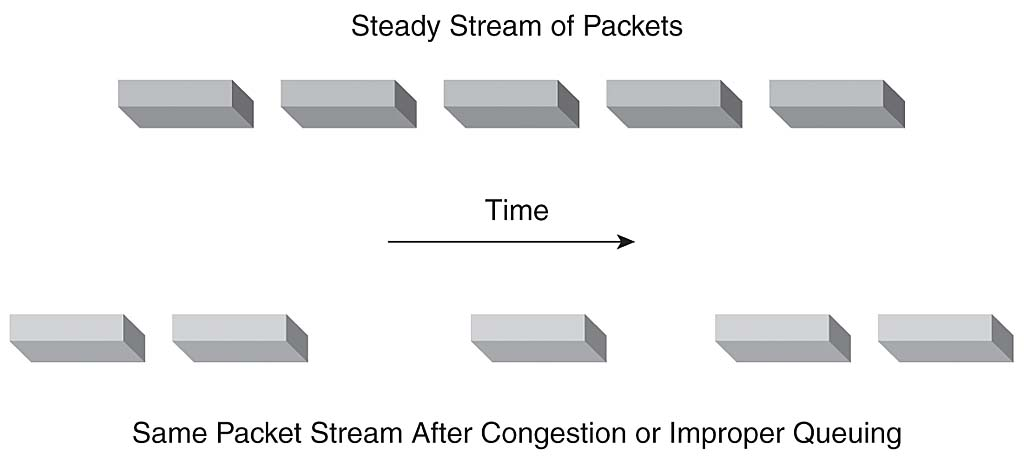
\includegraphics[width=\linewidth]{jitter}
	\caption{Wizualizacja zjawiska jitter, źródło: \cite{jitter}}
	\label{fig:jitter}
\end{figure}

Drugie zjawisko, jitter, zobrazowane zostało na rysunku \ref{fig:jitter}. Jitter występuje, gdy dane w sieciach pakietowych wysłane w równych odstępach czasu (górna część rysunku) docierają do odbiorcy w różnych odstępach czasu (dolna część rysunku). Wahania opóźnienia pakietów należących do tej samej transmisji mogą być spowodowane obciążeniem sieci lub wyborem różnych ścieżek dla tych danych przez urządzenia sieciowe. Na jitter podatne są przede wszystkim aplikacje pozwalające na komunikację głosową. W sieciach w których działają takie aplikacje zwykle  wdrożone jest Quality of Service. Dzięki temu dane głosowe otrzymują wysoki priorytet i są przekazywane przez urządzenia sieciowe w pierwszej kolejności. Zmniejsza to zarówno opóźnienie jak i jitter dla transmisji głosowych. W celu dalszego zmniejszenia wpływu jitter na działanie transmisji, implementowane są bufory w aplikacji klienta. Takie rozwiązanie pozwala na powtórne ``wygładzenie'' strumienia pakietów, ale zwiększa całkowite opóźnienie transmisji.

Utrata danych w sieciach komputerowych może nastąpić z wielu powodów. W warstwie fizycznej możliwa jest zmiana przesyłanych sygnałów wskutek interferencji zewnętrznych lub niedoskonałości samego medium. W przypadku warstwy łącza danych i najszerzej stosowanego standaru jakim jest Ethernet utrata ramki może być następstwem kolizji, niezgodności sumy kontrolnej CRC\footnote{Cyclic Redundancy Check - sposób tworzenia skrótu z danych obliczany w celu możliwości późniejszego ustalenia ich spójności.} z wartością policzoną na urządzeniu sieciowym lub pętli. Pętle w warstwie drugiej mogą doprowadzić do \textit{broadcast storms} i w rezultacie sprawić, że sieć będzie niedostępna. Z kolei w warstwie sieciowej utrata pakietów może nastąpić na skutek braku odpowiednich tras na urządzeniach pośredniczących w wymianie danych lub zaimplementowanych środków bezpieczeństwa (zapory, filtry, itd...). Innym możliwym powodem utraty danych są konfiguracje urządzeń sieciowych. Niepoprawne lub zbyt restrykcyjne polityki zaimplementowane na urządzeniach sieciowych mogą spowodować całkowitą lub częściową utratę danych i stanowić wyzwanie przy próbie poprawy działania tych urządzeń. Urządzenia ograniczające komunikacje mogą znajdować się pod kontrolą innego podmiotu administracyjnego, co dodatkowo komplikuje proces poprawy działania sieci.
\begin{figure}[h!]
	\centering
		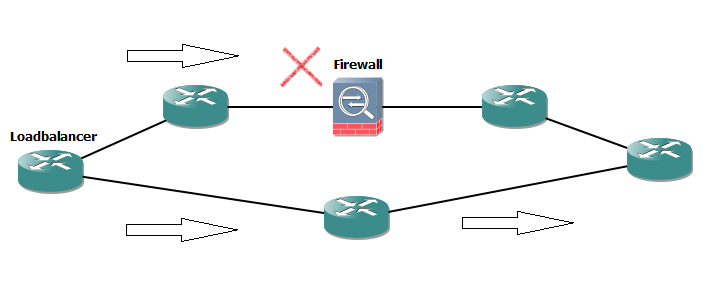
\includegraphics[width=0.9\linewidth]{drop}
	\caption{Błędna konfiguracja urządzeń sieciowych powoduje częściową utratę danych.}
	\label{fig:drop}
\end{figure}
Rysunek \ref{fig:drop} przedstawia przykład w którym konfiguracja urządzeń powoduje częściową utratę danych. Loadbalancer równoważy obciążenie pomiędzy dwoma trasami. Na górnej trasie znajduje się zapora, która filtruje ruch i rezultacie tylko część pakietów (przesłana trasą dolną) dociera do odbiorcy. 

Również w warstwie sieciowej mogą występować pętle i protokoły działające na tym poziomie powinny być wyposażone w mechanizmy pozwalające na usuwanie danych krążących w takich pętlach. W przypadku protokołu IP zdefiniowane jest pole TTL (Time to live) określające maksymalną liczbę urządzeń sieciowych, które mogą przetworzyć pakiet zanim dotrze on do odbiorcy. Przy każdym przetworzeniu pakietu przez urządzenie wartość pola jest zmniejszana o 1 (maksymalna wartość tego pola to 255) i jeżeli spanie do 0 to pakiet jest usuwany z sieci.

\section{Zmienność warunków panujących w sieciach komputerowych}

Szybkość transmisji danych zależy bezpośrednio od przepustowości łączy znajdujących się pomiędzy nadawcą i odbiorcą. Do sieci zwykle podłączonych jest wielu użytkowników wymieniających pomiędzy sobą dane, często w sposób nieregularny. Część łączy pomiędzy użytkownikami musi być współdzielona, co oznacza, że całkowita dostępna przepustowość na tych łączach może być zmienna w czasie. Zakres i częstotliwość z jaką zmienia się dostępne pasmo zależy od charakteru transmisji danych prowadzonych przez użytkowników, a utraty danych i ich retransmisje prowadzą do jeszcze większych nieregularności przepustowości sieci.

\begin{figure}[h!]
	\centering
		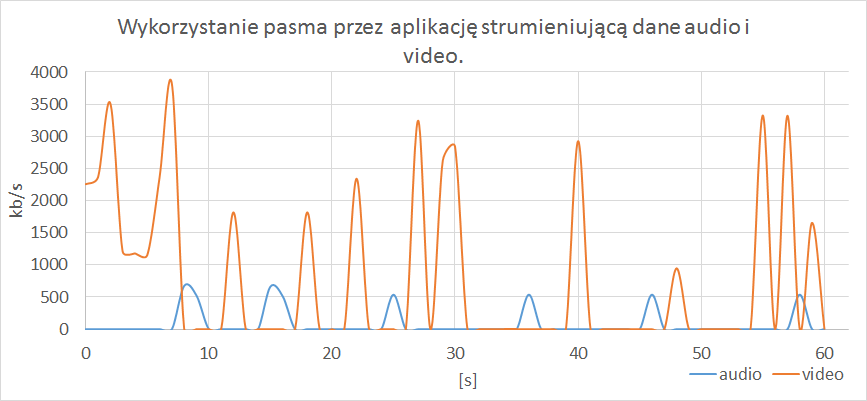
\includegraphics[width=\linewidth]{audiovideobitrate}
	\caption{Porównanie transmisji audio i video.}
	\label{fig:audiovideobitrate}
\end{figure}

Rysunek \ref{fig:audiovideobitrate} obrazuje różnice w transmisjach danych audio oraz video. Do testu wykorzystano dwa laptopy z kartami sieciowymi, przełącznicę Cisco Catalyst 3500 oraz oprogramowanie VLC i Wireshark. Laptopy i przełącznica zostały połączone w jedną sieć LAN.  Jeden z laptopów posłużył jako serwer HTTP na którym znajdowały się pliki multimedialne. Na drugim laptopie zainstalowano programy VLC\footnote{VLC to rozbudowany program do odtwarzania danych multimedialnych. Posiada funkcjonalność strumieniowania plików audio i video.} i Wireshark\footnote{Wireshark to tzw. \textit{Sniffer}, czyli program pozwalający na przechwycenie i rozkodowanie pakietów pojawiających się na interfejsie urządzenia.}. Wykres wygenerowano na podstawie informacji zgromadzonych przez Wireshark (funkcja~``IO Graphs'') w ciągu 60 sekund ciągłego strumieniowania danych za pomocą VLC.

Transmisje audio zajmują znaczne mniejszą część pasma i charakteryzują się stałym jego wykorzystaniem. Zajętość pasma dla transmisji video jest większa, zmnienna w czasie i zależy od sposobu kodowania przesyłanych danych. Plik video zwykle kodowany jest wewnątrz-ramkowo i między-ramkowo. Kodowanie wewnątrz-ramkowe pozwala na zmniejszenie wielkości pojedynczej ramki. Stopień kompresji zależy zarówno od cech ramki jak i od algorytmu kodującego. Kodowanie między-ramkowe polega zakodowaniu ramki na podstawie ramek sąsiadujących i pozwala na największy stopień kompresji, gdy obraz video pozostaje statyczny (kolejne ramki są prawie identyczne lub bardzo podobne).

Poza charakterystyką przesyłanych danych na transmisję mogą wpływać cechy protokołów z których ta transmisja korzysta. Protokoły wykorzytywane przez aplikacje do komunikacji w sieci należą do warstwy transportowej i mogą zostać sklasyfikowane według kilku kategorii. Pierwszy rodzaj podziału dotyczy zachowania się protokołów w przypadku utraty danych. Protokoły niezawodne posiadają mechanizmy retransmisji utraconych danych i implementują liczniki czasu, po których upływie dane zostają uznane za zaginione. Dzięki temu dane są przekazywane w całości do odbiorcy, ale takie podejście powoduje dodatkowe narzuty na komunikację. Protokoły zawodne nie obsługują mechanizmów retransmisji i niedają żadnych gwarancji, że dane zostaną dostarczone do odbiorcy. Kolejny podział protokołów moża przeprowadzić ze względu na sposób inicjalizacji komunikacji i jej zakończenia. Protokoły połączeniowe przed wysłaniem danych nawiązują połączenie w celu ustalenia, czy odbiorca jest gotowy do przyjęcia przesyłanych danych. W trakcie inicjalizacji połączenia możliwa jest wymiana wartości parametrów w celu usprawnienia dalszej komunikacji. Protokoły bezpołączeniowe nie sprawdzają dostępności odbiorcy. Ich rola polega jedynie na wysłaniu danych do ustalonego adresata, bez względu na to czy jest w stanie te dane odebrać, czy też nie. Brak możliwości sprawdzenia dostępności adresata może prowadzić do przesyłania danych, które nie mogą zostać odebrane. Kolejne dwie kategorie dotyczą zachowania się protokołów w przypadku przeciążenia sieci lub odbiorcy. Protokoły reagujące na zwiększony ruch w sieci implementują mechanizmy kontroli przeciążeń. Jeżeli protokół wykryje, że sieć jest przeciążona to ograniczy szybkość z jaką przesyła dane. Protokoły nie implementujące kontroli przeciążeń zachowują się bardziej agresywnie przy konkurowaniu o dostępne pasmo, jednak w przypadku wykorzystania całej dostępnej przepustowości możliwa jest utrata dużej części przesyłanych danych - istnieje ryzyko, że urządzenia sieciowe odrzucą dane, ponieważ nie nadążają z ich przetwarzaniem. Z kolei mechanizmy kontroli przepływu zabezpieczają odbiorców przed zalaniem danymi. Jeżeli urządzenie nadawcy wysyła dane szybciej niż urządzenie odbiorcy jest w stanie je odebrać to istnieje ryzyko przepełnienia buforów po stronie odbierającej. Taka sytuacja jest niepożądana, ponieważ może doprowadzić do utraty danych i pogorszenia jakości transmisji.

\section{Wpływ konfiguracji urządzeń sieciowych na strumienie danych}

Konfiguracja Quality of Service może wywierać znaczący wpływ na jakość i szybkość przesyłania danych. QoS to zbiór usług pozwalających na:
\begin{itemize}
\item priorytetyzację wybranych klas ruchu,
\item kontrolę opóźnienia,
\item kształtowanie dostępnego pasma,
\item wybór sposobu odrzucania danych.
\end{itemize}

Kontrola opóźnienia i priorytetyzacja ruchu jest możliwa poprzez klasyfikację ruchu oraz zastosowanie różnych polityk dla różnych klas ruchu. Klasyfikacja ruchu może odbywać się w oparciu o wykorzystywane protokoły lub aplikacje działające na dobrze znanych portach. Rozpoznanie protokołu na podstawie zawartości pojedynczego pakietu może okazać się niemożliwe (np. RTP), dlatego narzędzia wykorzystywane w tym celu analizują grupy pakietów. Porównując różnice w nagłówkach kolejnych pakietów możliwe jest ustalenie z pewnym prawdopodobieństwem protokołu używanego w danej transmisji. Przykładem narzędzia działającego w ten sposób jest Network Based Application Recognition (NBAR) firmy Cisco. Po zaklasyfikowaniu ruchu, urządzenie sieciowe obsługuje dane zgodnie z zaimplementowanymi politykami. Polityki mogą określać kolejność obsługi danych przez urządzenie, kolejność ich odrzucania w przypadku przeciążenia oraz wpływać na opóźnienie wywołane dużym ruchem w sieci. Rysunek \ref{fig:qosmodel} przedstawia referencyjny model QoS. Dane znajdujące się wyżej powinny posiadać wyższy priorytet od danych znajdujących się niżej w hierarchi i być obsługiwane w pierwszej kolejności. Podział ten wynika z faktu, że dane czasu rzeczywistego (rozmowy telefoniczne, video-konferencje) są wrażliwe na jitter, opóźnienie i utratę pakietów. Ruch generowany przez protokoły routingu i dotyczący zarządzania siecią również wymaga szybszej obsługi, co przyspieszy konwergencję sieci. Dane typu best effort oraz bulk do których należy zdalne tworzenie kopii zapasowych nie nakładają ograniczeń na jitter i opóźnienie. Dlatego też mogą być obsługiwane z niższym priorytetem.

\begin{figure}[h!]
	\centering
		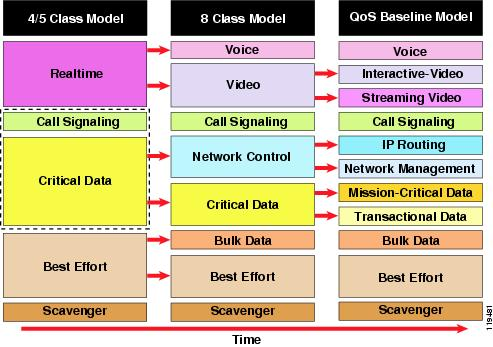
\includegraphics[width=0.7\linewidth]{qosmodel}
	\caption{Referencyjny model Quality of Service}
	\label{fig:qosmodel}
\end{figure}

Zmniejszanie lub zwiększanie dostępnej przepustowości może odnosić się do całego ruchu przechodzącego przez urządzenie sieciowe, bądź tylko do konkretnych klas tego ruchu. Przykładowo możliwe jest ograniczenie ruchu nie posiadającego kontroli przeciążeń w celu usprawnienia transmisji reagujących na zmiany w dostępnym paśmie. Implementacja polityki tego typu pozwoli na zapewnienie bardziej stabilnego podziału łącza pomiędzy transmisje wykorzystujące zróżnicowane protokoły.

\begin{figure}[h!]
	\centering
		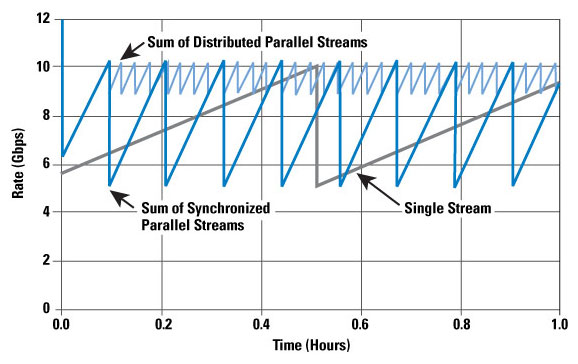
\includegraphics[width=0.7\linewidth]{tcpsynchro}
	\caption{Problem synchronizacji strumieni.}
	\label{fig:tcpsynchro}
\end{figure}

Mechanizmy decydujące o odrzucaniu części przychodzących danych ze względu na zbyt duże natężenie ruchu również mogą wywierać znaczny wpływ na transmisje danych. W najprostszym przypadku, gdy urządzenie nie nadąża z przetwarzaniem informacji, dane są odrzucane. Takie zachowanie może prowadzić do niepożądanych zjawisk. Jednym z takich zjawisk jest synchronizacja strumieni TCP zobrazowana na rysunku \ref{fig:tcpsynchro}.

TCP wykorzystuje mechanizmy kontroli przepływu i przeciążeń w celu zabezpieczenia sieci i odbiorców przed przeciążeniem. Mechanizmy te nadają transmisji specyficzny charakter. Z upływem czasu dane do strumienia wkładane są z coraz większą szybkością, a w chwili wykrycia przeciążenia szybkość ta gwałtownie spada (pojedynczy strumień na rysunku \ref{fig:tcpsynchro}). Jeżeli w sieci działa kilka strumieni i każdy z nich zacznie tracić dane w tym samym momencie to wspomniane mechanizmy ulegną synchronizacji i nie będzie możliwe pełne wykorzystanie dostępnego pasma (suma zsynchronizowanych strumieni na rysunku \ref{fig:tcpsynchro}). Ryzyko globalnej synchronizacji strumieni można niwelować poprzez zastosowanie mechanizmu Random Early Detection (RED) zaprezentowanego na rysunku \ref{fig:red}.

\begin{figure}[h!]
	\centering
		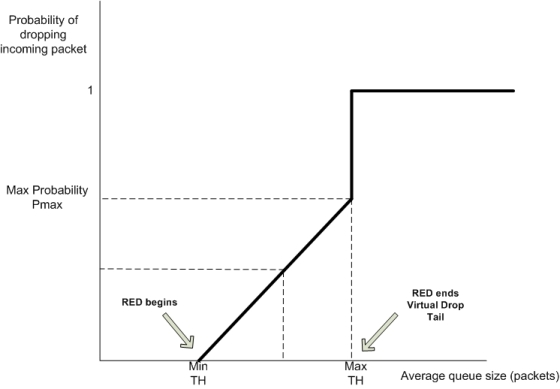
\includegraphics[width=0.8\linewidth]{red}
	\caption{Mechanizm Random Early Detection, źródło \cite{red-mechanism}}
	\label{fig:red}
\end{figure}

Mechanizm RED bazuje na długości kolejki (bufora) interfejsu urządzenia sieciowego. Jeżeli ilość danych w kolejce przekroczy wartość Min TH (minimum threshold) to rozpoczyna się proces odrzucania części danych. Dane mogą zostać odrzucone z liniowym prawdopodobieństwem określonym na podstawie zajętości kolejki. Jeżeli długość kolejki przekroszy Max TH (maximum threshold) wszystkie dane pojawiające się na interfejsie zostaną odrzucone. Probabilistyczne podejście do odrzucania danych zapobiega synchronizacji mechanizmów kontroli i pozwala na lepsze wykorzystanie dostępnego pasma.

\section{Dostarczanie danych do wielu odbiorców}

Jeżeli transmisja powinna zostać dostarczona do wielu odbiorców to wykorzystanie komunikacji punkt-punkt jest niewydajne. Pakiety przenoszące informacje muszą być powielane i adresowane do każdego z odbiorców osobno. W celu poprawy wykorzystania łącza możliwe jest skorzystanie z technologii multicast, dzięki której transmisja może dotrzeć do wielu odbiorców bez zbędnego przesyłania tych samych inforamcji wielokrotnie przez to samo łącze. 

Najbardziej rozpowszechnionymi protokołami pozwalającymi na transmisje multicast są Protocol Independent Multicast (PIM) oraz Internet Group Management Protocol (IGMP). Protokół IGMP pozwala użytkownikom na powiadamianie urządzeń sieciowych o zamiarze przyłączenia się lub odejścia\footnote{Powiadamianie o opuszczaniu grupy jest dostępne od drugiej wersji protokołu IGMP.} z grupy multicast. Informacje uzyskane z protokołu IGMP oraz z protokołów routingu unicast są wykorzystywane przez PIM do budowy drzewa rozpinającego sieć w której działa (zob. rysunek \ref{fig:pim}). PIM może działać w kilku z poniżej przedstawionych trybów:
\begin{itemize}
\item Sparse mode - polega na budowie współdzielonego drzewa (ST) dla grupy, którego korzeniem jest RP (Rendezvous Point). Zapewnia dobre skalowanie w dużych sieciach.
\item Dense mode - polega na budownie najkrótszego drzewa (SPT) poprzez zalewanie, a następnie odcinanie gałęzi sieci w których nie ma odbiorców.
\item Source specific mode - tryb pozwalający na odbiór transmisji grupowej od konkretnego źródła.
\end{itemize}

\begin{figure}[h!]
	\centering
		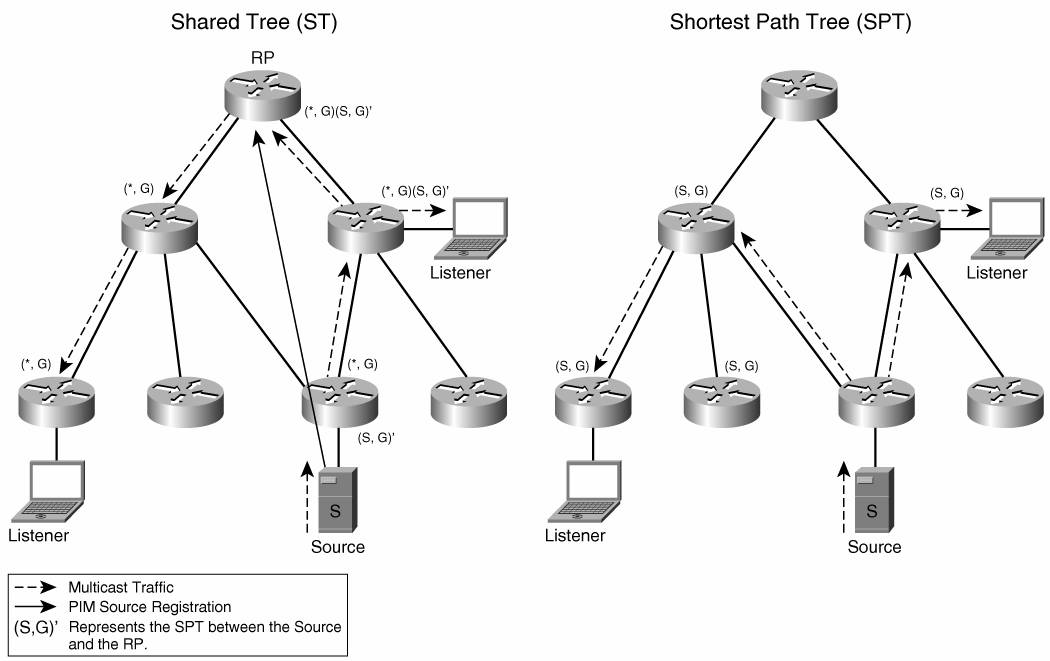
\includegraphics[width=\linewidth]{pim}
	\caption{Drzewa budowane przez różne tryby protokołu PIM.}
	\label{fig:pim}
\end{figure}

Znaczącą wadą tego rozwiązania jest fakt, że Internet obecnie nie jest przystosowany do przesyłania danych multicast na szeroką skalę. Implementacja tej technologii zajmuje zasoby na urządzeniach sieciowych i wymaga protokołów routingu i kontrolowania położenia odbiorców w sieciach (PIM, IGMP). Kolejny problem w transmisji grupowej stanowi brak możliwości wyboru danych do strumieniowania po stronie klienta. Klient nie może ponownie odtworzyć fragmentu meczu, który dopiero obejrzał lub przewinąć części strumieniowanego filmu do przodu. Możliwe jest jednak udostępnienie klientowi tych funkcjonalności przy użyciu serwerów cache i odtwarzaczy buforujących otrzymywane dane.

Innym podejściem do strumieniowania danych charakteryzują się protokoły typu P2P (Peer-to-peer). W rozwiązaniach opartych na tej technologi nie ma ``wąskich gardeł'' w postaci centralnych serwerów. Dane znajdujące się u jednego lub więcej użytkowników mogą być bezpośrednio przesłane do odbiorcy. Każdy odbiorca może strumieniować dane od wielu użytkowników, co pozwala na rozłożenie obciążenia sieci i stacji wysyłających. To podejście również ma swoje wady w szczególności dotyczące bezpieczeństwa i jakości danych które odbiorca otrzymuje. 

\section{Podsumowanie}

W powyższym rozdziale opisano zjawiska związane z transmisją danych w sieciach komputerowych (jitter, opóźnienie, utrata pakietów) oraz wyjaśniono dlaczego sieci charakteryzują się zmniennością dostępnego pasma. Przedstawiony został wpływ konfiguracji urządzeń sieciowych na strumieniowanie danych oraz podejścia, które można zastosować w przypadku strumieniowania tych samych danych do wielu odbiorców.

Strumieniowanie adaptacyjne, polegające na dostosowaniu bitrate danych multimedialnych do warunków panujących w sieci ma znaczą przewagę nad pozostałymi technologiami - nie jest ograniczone przez zasięg administracyjny organizacji. Technologie Quality of Service i multicast wymagają implementacji na wszystkich urządzeniach pomiędzy nadawcą i odbiorcą. Nie istnieje jednak wymóg implementacji tych technologii i sieci należące do ISP zwykle nie udostępniają takich funkcjonalności. Natomiast strumieniowanie adaptacyjne wymaga jedynie wsparcia ze strony serwera oraz aplikacji klienta i działa w sposób transparentny dla pośrednich urządzeń sieciowych.